\documentclass[10pt]{style}
\usepackage[centertags]{amsmath}
\usepackage{amsthm}
\usepackage{epsfig}

% THEOREMS ---------------------------------------------------------------
\theoremstyle{plain}
\newtheorem{thm}{Theorem}
\newtheorem{cor}[thm]{Corollary}
\newtheorem{lem}[thm]{Lemma}
\newtheorem{prop}[thm]{Proposition}

\theoremstyle{definition}
\newtheorem{defn}{Definition}%[section]

\theoremstyle{remark}
\newtheorem{rem}{Remark}[section]

\numberwithin{equation}{section}
\renewcommand{\theequation}{\thesection.\arabic{equation}}

\title {Butterfly Network Reliability}
\author {Aydan R. Yumerefendi}
\begin{document}

  \maketitle

  We examine the problem of Butterfly network
  reliability. Let $B$ be a butterfly network of degree 2 with $n$
  nodes total, such that all are present on each level.  We label the
  levels of $B$ staring from 0 to $\log_2n$, where 0 is the input
  level. The basic property of the  so defined Butterfly network is
  that any of its inputs is eventually propagated 
  to all network nodes. Let's assume that each input is initially provided
  to $c \geq 1$ independently chosen random nodes on level 0. We will
  study the probability that a Butterfly node on a given level
  receives a particular input.

  {\bf No Failures.} Assume that no node of $B$ fails before $B$ has
  completed its operations. Let $A$ be the event that a given node is
  the first chosen to receive a particular value on level 0. Clearly $P(A) =
  \frac{1}{n}$ and $P(\overline{A}) = \frac{n-1}{n}$. Let $B$ be the
  event that a node on level 0 was not chosen to receive a particular
  value after all $c$ trials. We have that $P(B) =
  (\frac{n-1}{n})^c$ and $P(\overline{B}) = 1-(\frac{n-1}{n})^c$.

  Let $P(k,n,c)$ be the probability that a node on level $k$ of a
  Butterfly network with $n$ nodes does not
  receive a particular value sent initially to $c$ randomly selected
  input nodes. We computed $P(0,n)$ to be $(\frac{n-1}{n})^c$. In
  general, a node $a$ does not receive value on level $k  > 0$ if $a$
  did not receive the value on level $k-1$ and if $b$ is the node $a$
  communicates with on level $k$, then $b$ also did not receive the
  value on level $k-1$. We can express this probability as: 

  \begin{eqnarray*}
    P(k,n,c) = P(k-1,n,c)P(k-1, n-2^{k-1},c)
  \end{eqnarray*}
  Where the first factor is the probability that $a$ did not receive
  the value, and the second factor is the probability that $b$ did not
  receive the value.

  For $k =1$, we have that:
  \begin{eqnarray*}
    P(1, n,c) &=& P(0, n,c)P(0, n-1,c) = \\
    &=&(\frac{n-1}{n})^c(\frac{n-2}{n-1})^c=\\
    &=&(\frac{n-2}{n})^c
  \end{eqnarray*}

  \begin{prop}
    $P(k,n,c) = (\frac{n-2^k}{n})^c$
  \end{prop}

  \begin{proof}
    We demonstrated that the above statement holds for $k=1$. Let
    for $k=l \leq 1$ the statement also be true. For $k=l+1$, we have:
    \begin{eqnarray*}
      P(l+1,n,c) &=& P(l,n,c)P(l, n-2^{l},c) = \\
      &=& (\frac{n-2^l}{n})^c(\frac{n-2^{l}-2^{l}}{n-2^l})^c =\\
      &=& (\frac{n-2^{l+1}}{n})^c
    \end{eqnarray*}
    $\Rightarrow P(k,n,c) = (\frac{n-2^k}{n})^c$ for any $0 \leq k
    \leq \log_2n$. 
  \end{proof}

  \begin{figure}
    \begin{center}
      \epsfig{file=figs/no_fail.eps,width=120mm}
      \caption{\footnotesize Probability of not receiving a value for
      each level of a Butterfly network with 1024 nodes, no failures, and varying
      replication factor $c$.}
      \label{test}
    \end{center}
  \end{figure}

  {\bf Independent Failures.}
  Assume that each Butterfly node can fail independently with
  probability $\epsilon$. We will compute $P(k,n,c)$ by conditioning
  on the event of a node failing. Let $A$ be the event that a node has
  not failed. We have that:
  \begin{eqnarray*}
    P(k,n,c) &=& P(k,n,c|A)P(A) +
    P(k,n,c|\overline{A})P(\overline{A})\\
    P(k,n,c|\overline{A}) &=& 1\\
    P(A) &=& 1-\epsilon\\
    P(\overline{A})&=& \epsilon      \\
    \Rightarrow P(k,n,c) &=& P(k,n,c|A)(1-\epsilon) + \epsilon
  \end{eqnarray*}
  A non failed node at level $k > 0$ does not receive a given value if
  it did not receive it at level $k-1$ and either talked to a
  non-failed node that also did not receive the value at level
  $k-1$ or talked to a failed node.Therefore:
  \begin{eqnarray*}
    P(k,n,c|A) &=& P(k-1,n,c|A)(\epsilon +\\
    &&(1-\epsilon)P(k-1,n-2^{k-1},c*|A))
  \end{eqnarray*}
  where $P(k-1,n-2^{k-1},c*|A)$ is the probability that the other good
  node did not receive the given value. We use $c*$ to denote the fact
  that it is unclear what value of $c$ should be used. Let $P'(k, n,
  c)$ be the probability that two non-failed nodes that communicate on level
  $k$ have not received a given value. Let also $P(B_i^k)$ be the
  probability that in the initial distribution of the given value,
  there have been $i$ selections in the first $2^k$ Butterfly
  nodes. We have:
  \begin{eqnarray*}
    P'(k, n, c) = \sum_{i=0}^{i=c}P(k-1,2^{k-1},i|A)P(k-1, n-2^{k-1}, c-i|A)P(B_i^{k-1})
  \end{eqnarray*}

  Let $X_{n,c}^k$ be a random variable describing the number of
  selections in the first $2^k$ nodes of a network of $n$ total nodes
  and replication factor $c$. We have that:
  \begin{eqnarray*}
    P(X_{n,c}^0=i) = {c \choose i}(\frac{1}{n})^i(\frac{n-1}{n})^{c-i} 
  \end{eqnarray*}
  We can define $P(X_{n,c}^k=i)$ recursively as:
  \begin{eqnarray*}
    P(X_{n,c}^k=i) = \sum_{j=0}^{j=i}P(X_{n,c}^{k-1}=
    i-j)P(X_{n-2^{k-1},c-i+j}^{k-1}= j)
  \end{eqnarray*}

  \noindent Therefore:
  \begin{eqnarray*}
    P(k,n,c|A) = \epsilon P(k-1,n,c|A) + (1-\epsilon)P'(k,n,c)
  \end{eqnarray*}
   
  \begin{figure}
    \begin{center}
      \epsfig{file=figs/with_fail_0_1.eps,width=120mm}
      \caption{\footnotesize Probability that a non-failed node will
      not receive a value for each level of a Butterfly network with
      1024 nodes, 0.1 failure rate, and varying replication factor $c$.}
      \label{test}
    \end{center}
  \end{figure}

  \begin{figure}
    \begin{center}
      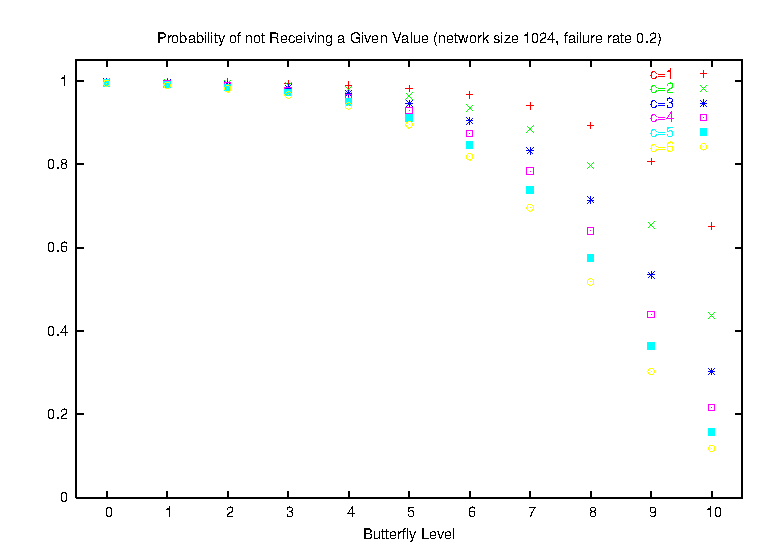
\epsfig{file=figs/with_fail_0_2.eps,width=120mm}
      \caption{\footnotesize Probability that a non-failed node will
      not receive a value for each level of a Butterfly network with
      1024 nodes, 0.2 failure rate, and varying replication factor $c$.}
      \label{test}
    \end{center}
  \end{figure}

  
%  {\bf Fixed Number of Failures.}
% Assume that at most $\epsilon$ fraction of all Butterfly nodes have
%  failed. We want to compute $P(k,n,c)$. Unlike the previous scenario,
%  the probability of talking to a failed node is no longer independent
%  on the Butterfly level. 
  
\end{document}
